\begin{figure}[H]
  \centering
  \caption{U-Shape Dynamics at $t=500$ (California, Florida, Washington)}
  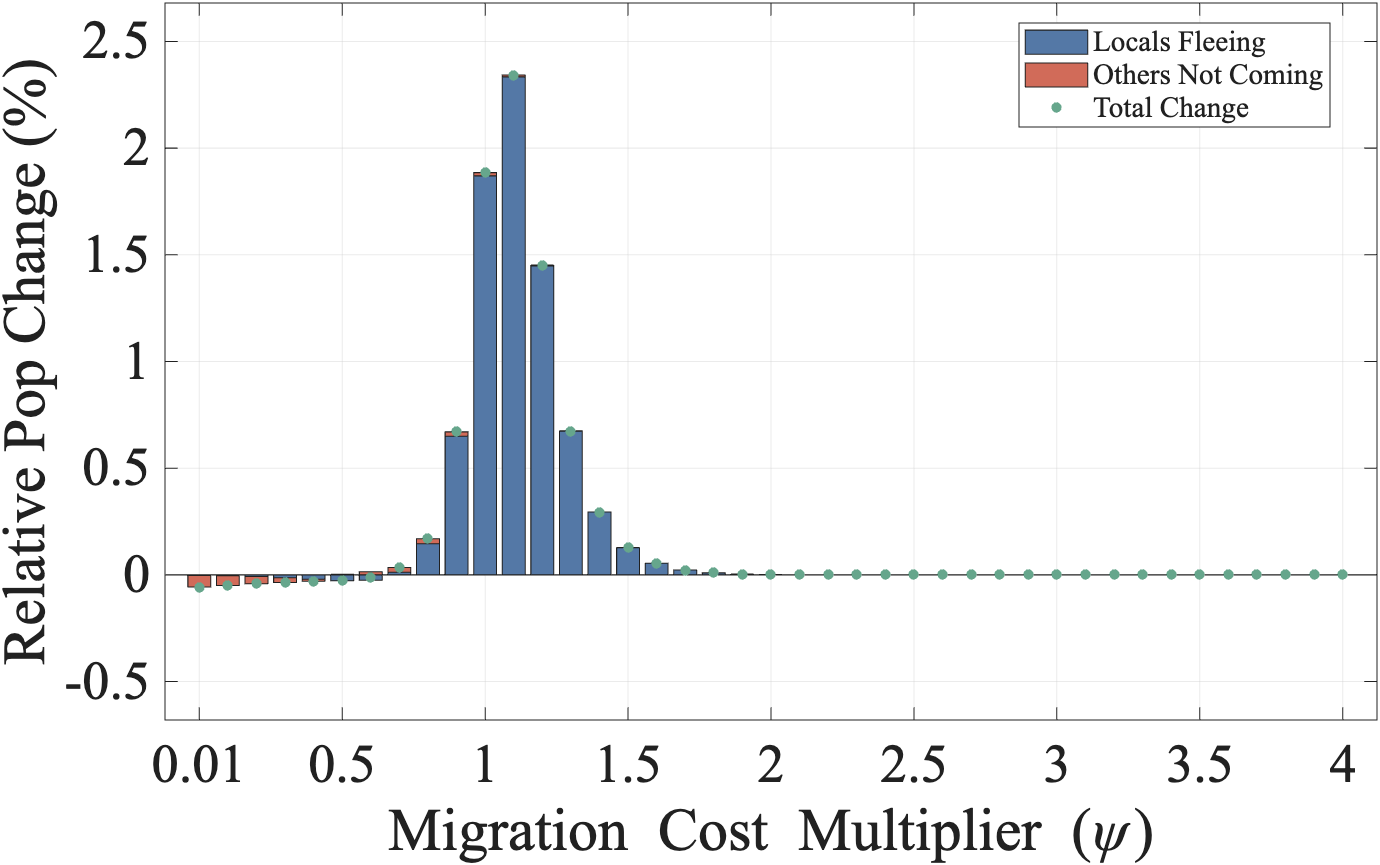
\includegraphics[width=0.65\textwidth]{../Output/small_nu/graph_ushape/ushape_t500_california.png} \\
  \small{(a) California} \\[2ex]
  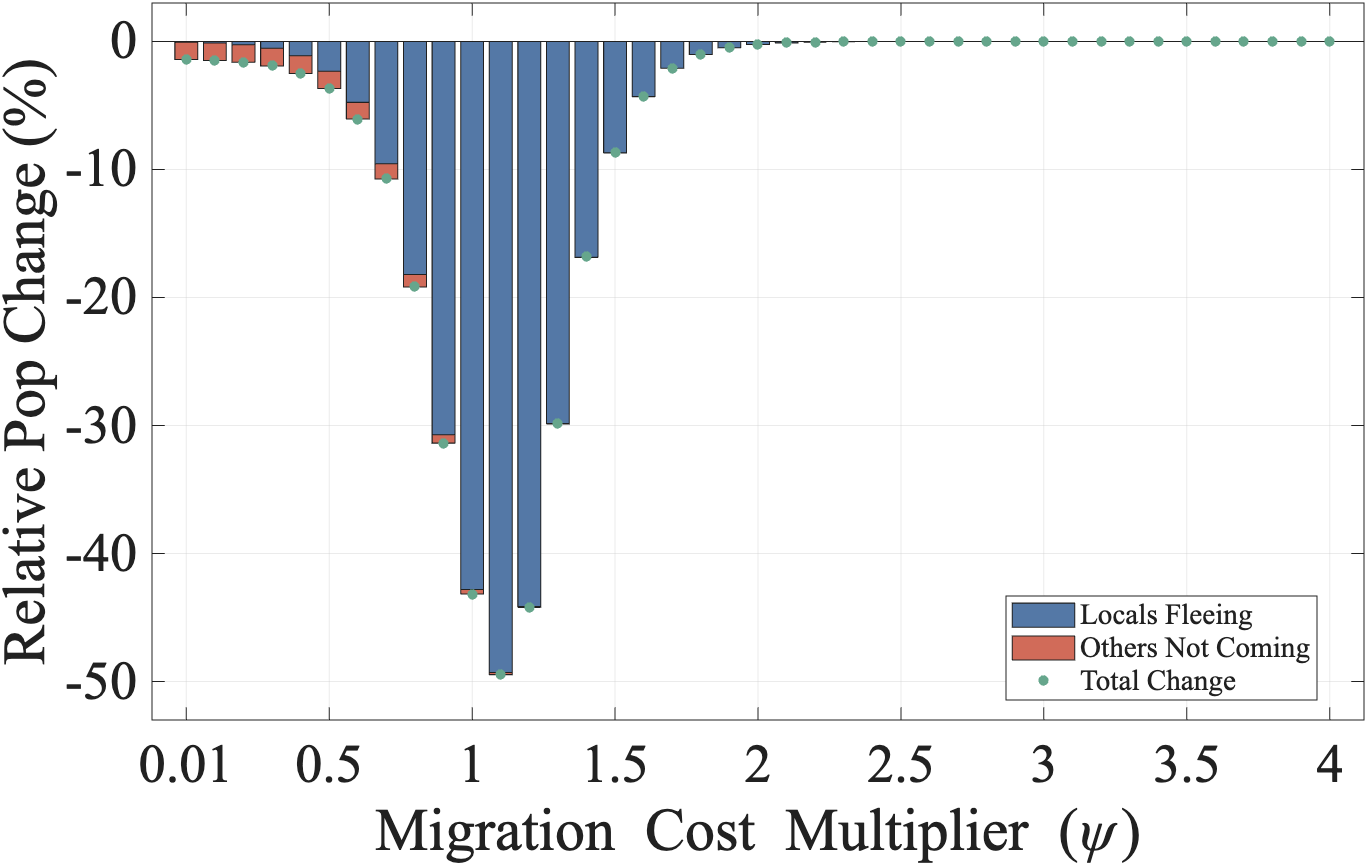
\includegraphics[width=0.65\textwidth]{../Output/small_nu/graph_ushape/ushape_t500_florida.png} \\
  \small{(b) Florida} \\[2ex]
  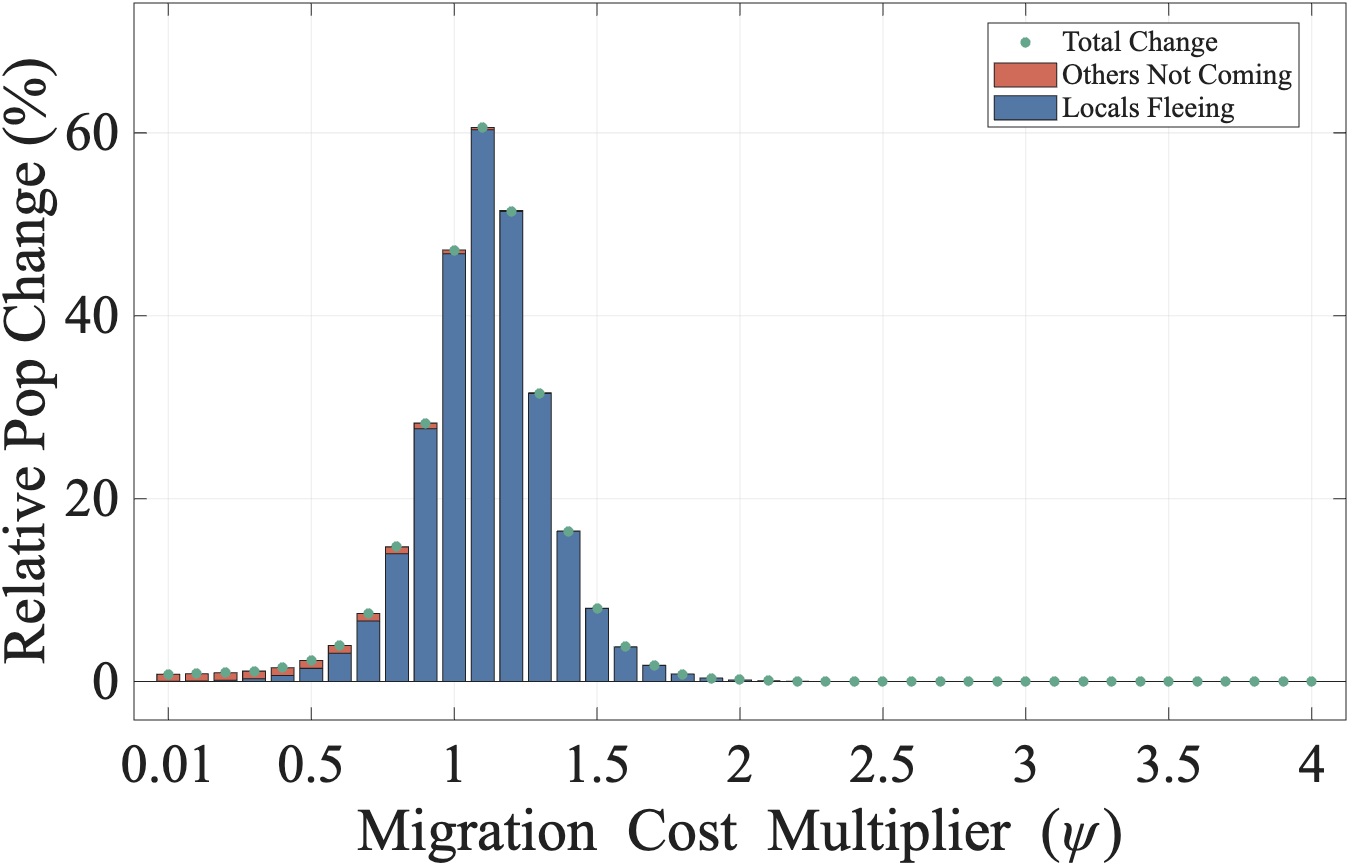
\includegraphics[width=0.65\textwidth]{../Output/small_nu/graph_ushape/ushape_t500_washington.png} \\
  \small{(c) Washington}
  \begin{minipage}{\textwidth}
  \vspace{0.5em}
  \footnotesize{\textbf{Note:} Long-run spatial sorting dynamics for major representative states for a wide range of migration costs exhibiting a U-shaped curve. Panels (a), (b), and (c) track population share trajectories $p_{\ell,t} = L_{\ell,t} / \sum_m L_{m,t}$ for California, Florida, and Washington.} \end{minipage}
\end{figure}